\begin{frame}
    \frametitle{Clustering the U-matrix}
    The main advantage of the flooding algorithm is to define cluster according to the flooding process.
    Each time the level goes down a new cluster is define.
    From this point of view we can define ``natural cluster'' without dealing with threshold definition!
    \begin{columns}
        \begin{column}{.4\textwidth}
            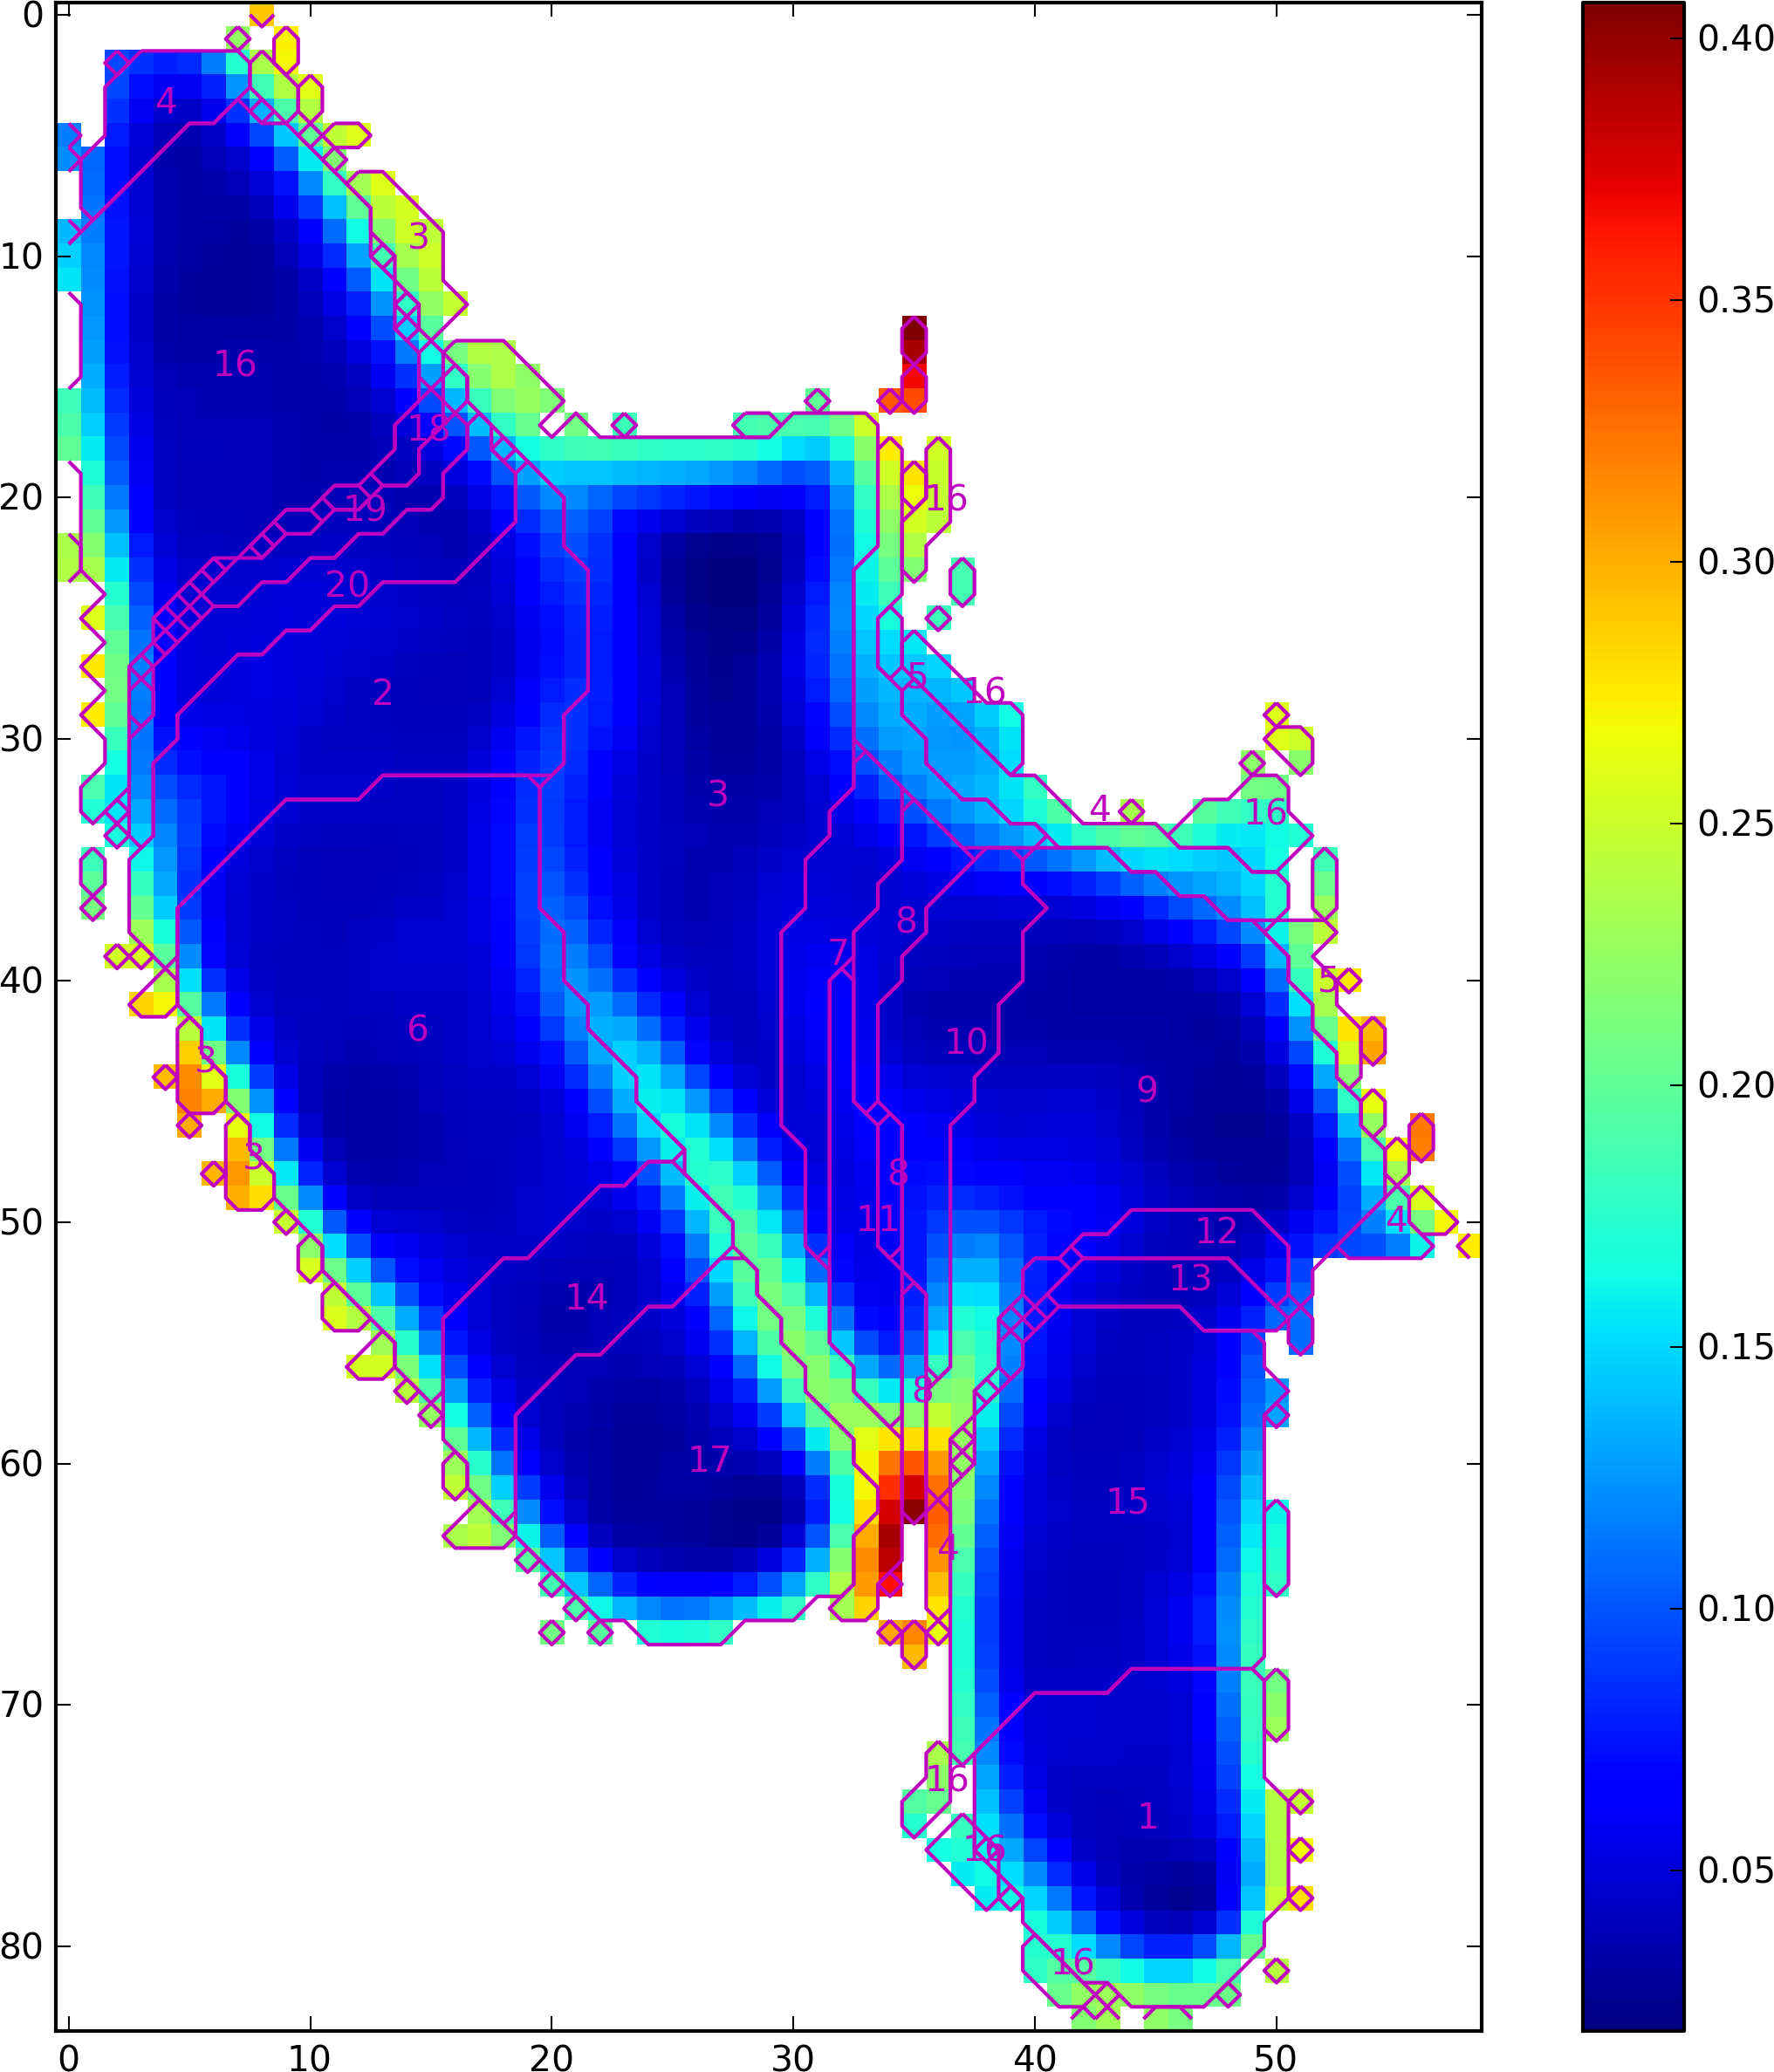
\includegraphics[width=\textwidth]{figures/umat_clust.png}
        \end{column}
        \begin{column}{.6\textwidth}
            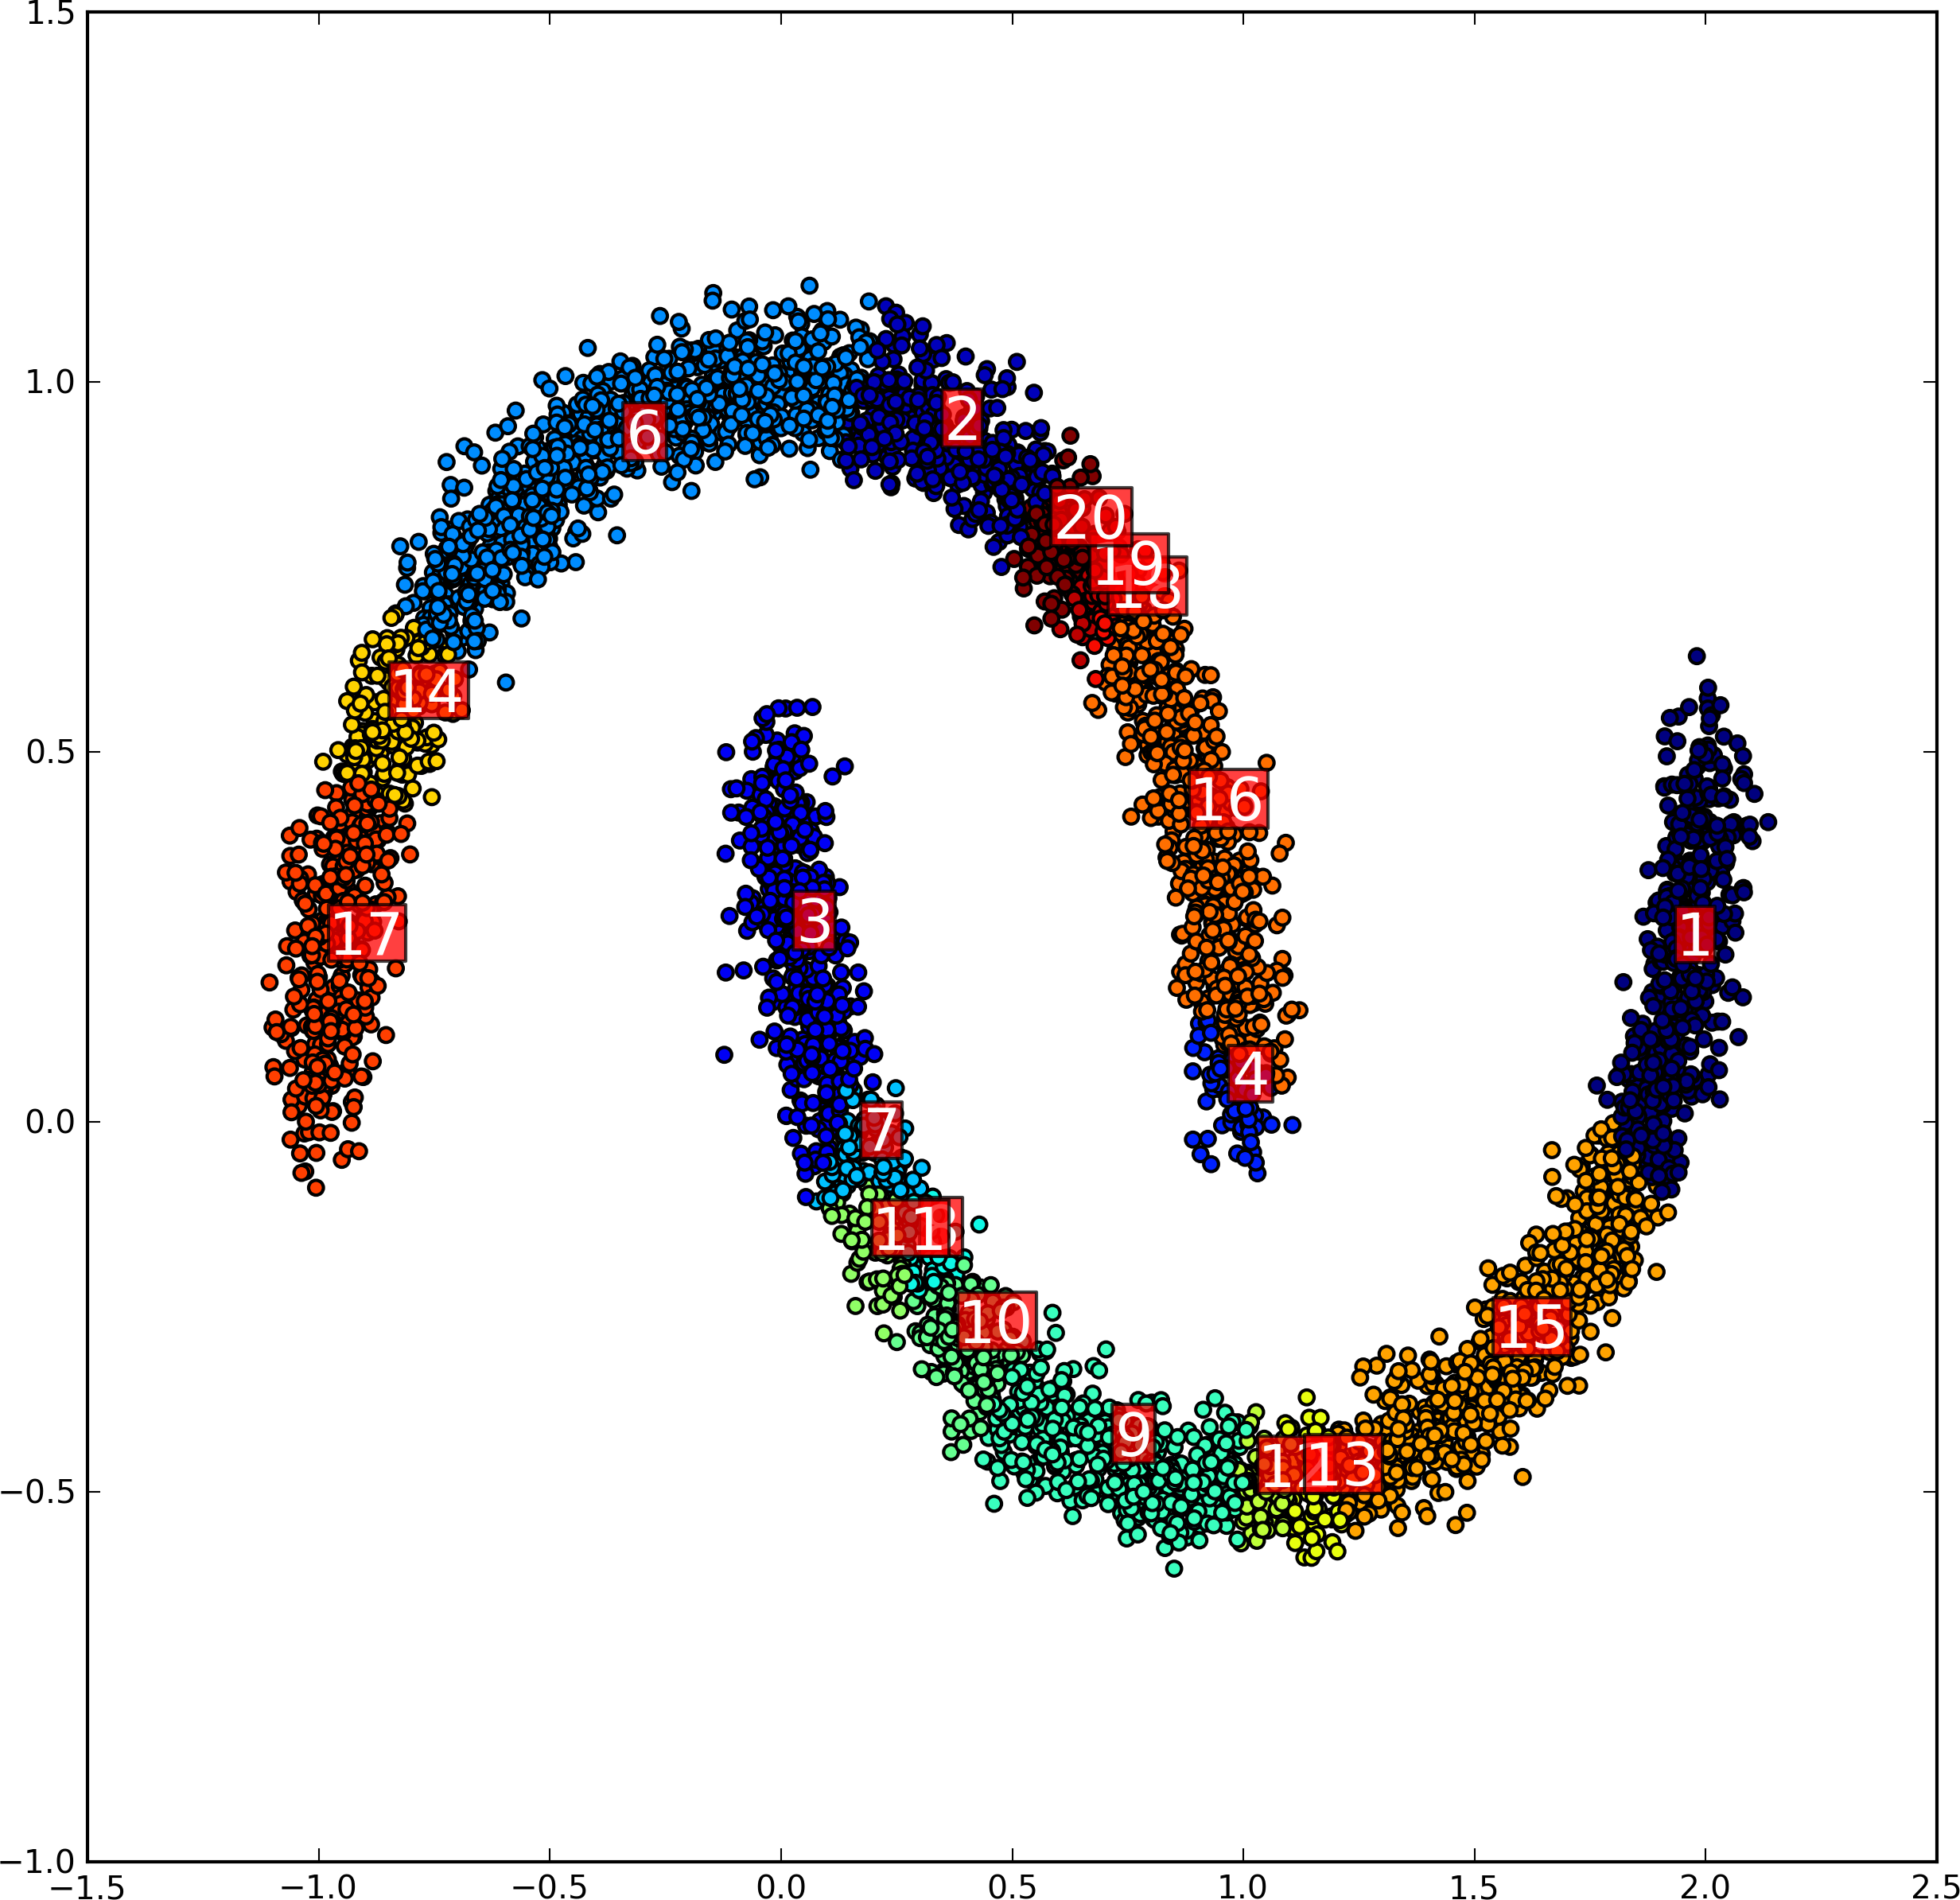
\includegraphics[width=\textwidth]{figures/moon_clust.png}
        \end{column}
    \end{columns}
\end{frame}
